\section{WebIDL Bindings} % (fold)
\label{sec:webidl_bindings}

In order to automatically generate stubs for JavaScript and C++ that allows communication between the two languages, an independent language, WebIDL, is used to define types and interfaces which will be used by both JavaScript and C++.

\begin{figure}
    \centering
    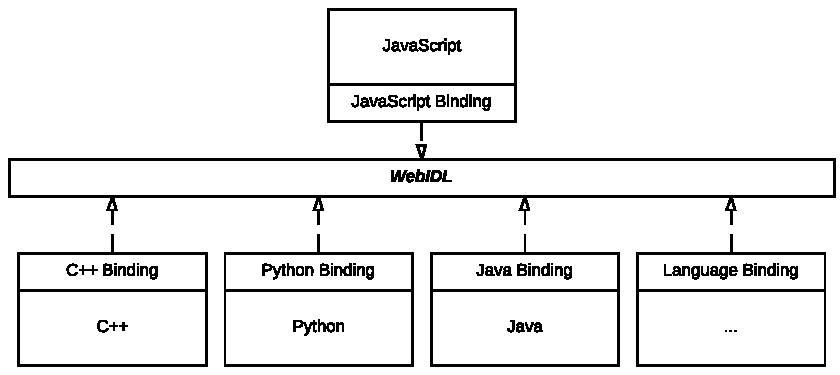
\includegraphics[width=1\textwidth]{JavaScript-WebIDL.pdf} 
    \caption{The WebIDL interface}
    \label{fig:webidl_intreface}
\end{figure}

The reason why this is needed is because JavaScript and C++ have entirely different type systems, and since the communication is two-way, we cannot simply map a C++ type into a JavaScript type. Moreover, if the RPC framework were to be completely language independent, we would need a mapping between every language's type into a JavaScript type. Therefore, to generalise, WebIDL gives an intermediary type interface so that other languages can communicate with JavaScript. The WebIDL types and syntax is defined as a standard, and gives EcmaScript bindings. In other words, the conversion between WebIDL and JavaScript types is defined in the standard. It is then up to the developer of the other language to define a binding from that language to WebIDL. This is illustrated in Figure \ref{fig:webidl_intreface}.

In this section, we mention the C++ WebIDL bindings used in the Native Calls project, and the design decisions behind them.

The implementation challenges involved in implementing these bindings are discussed at a later chapter.

\subsection{Modules, Interfaces, and Functions} % (fold)
\label{sub:modules_and_interfaces}
In Native Calls, we make a distinction between `modules' and `interfaces'. Essentially, a module contains several interfaces. And an interface contains several function definitions.

When we define a module, we must define all the interfaces, type definitions, and dictionaries for it in the same generator call. The definitions could be in different IDL files.

In JavaScript, a module is represented as an object which has a property for each interface that module defines. Therefore, each interface has a property for each function that interface defines. 

In C++, a module is represented as a class, which sets up the module. When setting up the module, each function interface is added. An IDL interface is represented by a C++ header file. The header file defines each function that is in the interface.

% subsection modules_and_interfaces (end)

\subsection{Number and String Types} % (fold)
\label{sub:number_types}
WebIDL defines a number of numeric types and also provides the JavaScript bindings for each type. Table \ref{table:webidl_cpp_numbers} shows the numeric types and their bindings in C++.

\begin{table}[h]
\centering
\begin{tabular}{l|lll}
\textbf{WebIDL Type} & \textbf{Min int} & \textbf{Max int} & \textbf{C++ Type}  \\ \hline
byte                 & $-2^{7}$         & $2^{7}-1$        & int8\_t            \\
octet                & $0$              & $2^{8}-1$        & uint8\_t           \\
short                & $-2^{15}$        & $2^{15}-1$       & int16\_t           \\
unsigned short       & $0$              & $2^{16}-1$       & uint16\_t          \\
long                 & $-2^{31}$        & $2^{31}-1$       & int32\_t           \\
unsigned long        & $0$              & $2^{32}-1$       & uint32\_t          \\
long long            & $-2^{63}$        & $2^{63}-1$       & int64\_t           \\
unsigned long long   & $0$              & $2^{64}-1$       & uint64\_t          \\
float                &                  &                  & float              \\
double               &                  &                  & double           
\end{tabular}
\caption{The C++ WebIDL bindings for number types}
\label{table:webidl_cpp_numbers}
\end{table}

It can be observed that the integer types are represented in C++ with the size information in it, even though C++ has equivalent type names for each of the WebIDL integer types. For example, C++ supports the \lstinline{short} type, but we explicitly decide to represent \lstinline{short} as \lstinline{int16_t}. The reason why explicit size information is included in the type is because of different implementations of certain types. For example, depending on the C++ standard library implementation we use, a \lstinline{long} can be represented in 32 bits or 64 bits. But because WebIDL explicitly defines the actual size of the integer types, to stick to the standard, we cannot tolerate this variation. For this reason, we use the explicit size types as shown above. This issue does not arise for \lstinline{float} and \lstinline{double} types as both C++ and JavaScript adhere to the IEEE 754 format.

Another interesting issue to note is that the bindings for large number types, such as \lstinline{long long}, are represented in JavaScript by the \emph{closest} numeric value. But because all JavaScript numbers are represented by 64 bit IEEE 754 (`double') types, the largest number that can be represented in JavaScript is actually $2^{53}-1$. This means that often the conversion between the WebIDL type and the JavaScript binding is \emph{lossy}, in the sense that it is not a one-to-one mapping. Although it would have been possible to overcome this issue by creating or using JavaScript `BigNumber' library classes, I decided to adhere to the specification, using the lossy conversion. This was for a few reasons:

\begin{itemize}
	\item Forcing the JavaScript user to use a number library is bad, as it adds more dependencies and is not conventional JavaScript e.g. the BigNumber library will have a different API to normal JavaScript numbers, and certain operations, such as addition, will not work properly.
	\item Using a different implementation, the RPC library could represent all data as \emph{binary}. JavaScript supports binary data in the form of ArrayBuffers.
	\item It is fairly unlikely that the developer would want to send back such large numbers to the JavaScript, and since the developer is developing for the web platform, they should be aware of JavaScript's limitations - including numeric type support.
\end{itemize}

To represent string types, the \lstinline{DOMString} WebIDL type is converted to the JavaScript \lstinline{string} type, as defined in the standard. As for the C++ binding, the \lstinline{std::string} class was chosen to represent DOMString. The alternative was to represent strings as character array buffers (\lstinline{char[]}). I decided to use the \lstinline{std::string} class for the following reasons:

\begin{itemize}
	\item JavaScript uses unicode (utf8) for strings. The developer would need to do some encoding/decoding to handle unicode characters, which may not fit in a byte.
	\item Simplicity: The PPAPI supports an \lstinline{AsString()} method on \lstinline{pp::Var} objects, which extracts the string value as a \lstinline{std::string} object.
	\item C++ developers use \lstinline{std::string} when they can. \lstinline{std::string} allows conversion to C strings using the \lstinline{c_str()} method.
\end{itemize}

% subsection number_types (end)

\subsection{Dictionary Types} % (fold)
\label{sub:dictionary_types}
The WebIDL standard defines the binding of a WebIDL dictionary to be a JavaScript Object with the keys being the identifier names of each dictionary member, and values being of the member's type. For example, Listing \ref{code_webidl_dictionary_example} shows an example of a dictionary definition in WebIDL and the corresponding JavaScript object according to the specification.

\lstset{language=JavaScript,caption={A WebIDL dictionary and its JavaScript binding},label=code_webidl_dictionary_example}
\begin{code}
// WebIDL
dictionary myObject {
  double id;
  DOMString name;
};

// Example JavaScript object
var myObj = {
  id: 31,
  name: "John Smith"
}
\end{code}

When a JavaScript object (and therefore a WebIDL dictionary) is sent to the NaCl module, it is represented in PPAPI as a \lstinline{pp::VarDictionary} object. \lstinline{pp::VarDictionary} allows extracting keys and values as \lstinline{pp::Var}. See background section \ref{sub:using_PPAPI} on page \pageref{sub:using_PPAPI} for more details.

We now consider how we can represent dictionaries in C++. The obvious approach is to represent a dictionary as a C \lstinline{struct}. The fields of the struct will have corresponding names and types as defined in the dictionary. For example, the struct shown in Listing \ref{code_webidl_struct_example} corresponds to the dictionary shown earlier in Listing \ref{code_webidl_dictionary_example}.


\lstset{language=C++,caption={A C struct corresponding to the dictionary definition in Listing \ref{code_webidl_dictionary_example}},label=code_webidl_struct_example}
\begin{code}
struct myObject {
  double id;
  std::string name;
}

// example use
struct myObject myObj;
myObj.id = 31;
myObj.name = "John Smith";
\end{code}


The advantage of this is that the object passed to the C++ programmer will be a normal C++ struct. However, it will impact performance, since each field of the struct will need to be individually converted. In fact, this makes marshalling dictionaries the slowest conversion, according to the benchmarks (see section \ref{sec:performance_evaluation}, page \pageref{sec:performance_evaluation}).

However, other approaches are possible. One alternative is we could have simply passed the \lstinline{pp::VarDictionary} object to the developer, without modifying it. The advantage of doing this is that it will simplify the C++ RPC library and therefore make it faster to send and receive complicated structures. However, there are a few problems with this approach:

\begin{itemize}
	\item The C++ developer is now exposed to PPAPI. This adds a learning curve, as it is another library that the C++ developer would have to get used to in order to write their module.
	\item The C++ developer will need to do all the type marshalling by themselves. This renders the dictionary type definition that they wrote in WebIDL useless, and adds more burden on the developer.
	\item The use of \lstinline{pp::VarDictionary} is actually an implementation detail of the RPC library. In other words, we simply use this as a way of transporting the data from JavaScript to C++. Perhaps someone could write another implementation that uses full binary transfer for example, using Protocol Buffers (see background section \ref{sec:data_representation_and_transfer}, page \pageref{sec:data_representation_and_transfer}). In that case, passing the \lstinline{pp::VarDictionary} to the developer would actually be more burden on the library, and probably impact performance.
\end{itemize}

Another approach is to represent a dictionary as a \lstinline{std::map}. The advantage of this is that the map can be added to and deleted from dynamically and unlike structs, if a field is not specified, data is not allocated for it. The problem with \lstinline{std::map} however is that the keys and values of the map have strict types. If the values have the same type, then a map will do fine; but what about if the values have different types, such as in the example in Listing \ref{code_webidl_dictionary_example}? The only way around this is by using wrapper types. For example, using \lstinline{pp::Var} again to represent the actual value, so the \lstinline{std::map} will be from \lstinline{std::string} keys to \lstinline{pp::Var} values. But again, this means the developer will have to de-marshal the \lstinline{pp::Var} to a standard library type, and this can get tedious when the value type is complex, for example, with multiple nested dictionaries.

In the end, we take the approach of individually, recursively de-marshalling the \lstinline{pp::VarDictionary} into a struct type, as a trade off of simplicity and developer friendliness to performance.
% subsection dictionary_types (end)

\subsection{Sequence Types} % (fold)
\label{sub:sequence_types}
In WebIDL, there are two ways of specifying a collection of types: sequence types (\lstinline{sequence<T>}) and array types (\lstinline{T[]}). The difference, according to the specification, is that a sequence type is \emph{passed by value} - meaning it is copied when passed into a function. Array types are passed by reference. 

Since \lstinline{postMessage} only transfers objects and values by value (i.e. structures are recursively copied), our RPC framework only supports sequence types. However, in JavaScript, they are represented in the same way (i.e. Array objects).

In C++, there are many ways of representing WebIDL sequence types, but we can assume that we have two options: using an array structure, or a standard library template class such as \lstinline{std::vector}. We compare each approach below.

The advantage of using an array is that we do not need to use an extra library, and it might be faster for large arrays. The problem of using arrays is that anywhere we use the array, we will need to also pass its length. This can get tedious, especially if we have a function that accepts many parameters. To overcome this, it is possible to send the length of the array with the actual array by augmenting the array after a designated terminator element, such as a NULL or zero element. For example, to specify the array \lstinline{[1,2,3,4]}, we send \lstinline{[1,2,3,4,NULL,4]}. The \lstinline{4} after the \lstinline{NULL} element is the length of the array. The problem with this, however, is that we need some kind of encoding scheme to ensure that the terminator and length elements do not get counted as actual array elements. For some array types, an encoding might not exist. Moreover, processing will need to be done in order for the developer to get the length of an array, thus the developer would need to get used to another library that is not standard C++.

The advantage of using a vector is that they are dynamic and they encapsulate the length of the vector. This means they are easy to both use and marshal. The disadvantage is that it forces the user to use the \lstinline{std::vector} library, especially in cases where the developer just wants an array.

In the end, I decided to go for the vector approach, for the following reasons:

\begin{itemize}
	\item The performance is nearly the same, since we allocate the size of the vector before using it. Also, regardless of the approach taken, it will take O(n) time to marshal and demarshal the array, since it needs to be converted to/from a \lstinline{pp::VarArray}.
	\item If the developer requires an array buffer, they can use the \lstinline{std::vector::data()} method to get a pointer to the vector's internal buffer.
	\item Vectors are generally how C++ developers represent collections of items, so most of the time it is fine to use the \lstinline{std::vector} library.
\end{itemize}

% subsection sequence_types (end)

\subsection{Implementation in C++} % (fold)
\label{sub:webidl_implementation_in_cpp_}
To implement WebIDL bindings in C++, we define how types are marshalled when sent and received from JavaScript. The IDL file will define \emph{what} types are expected, whilst the C++ implementation will define \emph{how} the types are accepted and received in the functions we define.

We already discussed the C++ bindings for number and string types. However, these types are sent and received from JavaScript as \lstinline{pp::Var} objects. To convert them, we define a generic \lstinline{RPCType} class, which has static \lstinline{AsVar} and \lstinline{Extract} methods. Other types then inherit from \lstinline{RPCType}. We define a type class for each WebIDL type. For example, Listing \ref{code_webidl_type_marshalling_long} shows the \lstinline{AsVar} and \lstinline{Extract} methods of the WebIDL long type.

\lstset{language=C++,caption={An example of WebIDL type marshalling},label=code_webidl_type_marshalling_long}
\begin{code}
pp::Var LongType::AsVar(const ValidType<int32_t>& v){
  return pp::Var((int) v.getValue());
}

ValidType<int32_t> LongType::Extract(const pp::Var& v){
  if(v.is_int()){
    return ValidType<int32_t>((int32_t)v.AsInt());
  } else {
    return ValidType<int32_t>();
  }
}
\end{code}

We do this for each WebIDL type. Now, complex types such as Dictionary and Sequence types use these classes to extract each of the keys and values of the dictionary. For example, Listing \ref{code_dict_marshal_xyz} shows how we convert a \lstinline{XYZ} dictionary type into an \lstinline{XYZ} struct or a \lstinline{pp::Var}. Notice how we use the \lstinline{Extract} methods of other WebIDL types, for example \lstinline{FloatType::Extract}. In this way, type extraction is recursive - it is simple to extract dictionaries which have values which are dictionaries, and so on. It also allows generating these classes simpler, since each type is \emph{only} concerned about extracting its own type, thus giving a general, uniform pattern for converting types. In fact, the code shown in Listing \ref{code_dict_marshal_xyz} is actually generated by our generator.

Notice also the use of the \lstinline{ValidType} class. This class is simply a wrapper over the C++ type. The reason we have it is to be able to check if a type is valid. If it is constructed without a value, then it is invalid. If it is constructed with a value, then it is valid. Therefore, we can check if the type marshalling and de-marshalling happened successfully by using the \lstinline{isValid} method on the \lstinline{ValidType} wrapper. We do this, for example, in the runtime layer, where we return an error if the type extraction failed, which can happen if an incorrect type was sent to the layer from JavaScript.

\lstset{language=C++,caption={An example of marshalling and de-marshalling a dictionary type called `\lstinline{XYZ}', which is defined to have three float members: \lstinline{x}, \lstinline{y}, and \lstinline{z}.},label=code_dict_marshal_xyz}
\begin{code}
ValidType<XYZ> XYZType::Extract(const pp::Var& v){
  ValidType<XYZ> invalid;
  if(v.is_dictionary()){
    pp::VarDictionary vDict(v);
    XYZ r;

    /* member: x */
    if(!vDict.HasKey("x")) return invalid;
    const ValidType< float >& xPart = FloatType::Extract(vDict.Get("x"));
    if(!xPart.isValid()) return invalid;
    r.x = xPart.getValue();

    /* member: y */
    if(!vDict.HasKey("y")) return invalid;
    const ValidType< float >& yPart = FloatType::Extract(vDict.Get("y"));
    if(!yPart.isValid()) return invalid;
    r.y = yPart.getValue();

    /* member: z */
    if(!vDict.HasKey("z")) return invalid;
    const ValidType< float >& zPart = FloatType::Extract(vDict.Get("z"));
    if(!zPart.isValid()) return invalid;
    r.z = zPart.getValue();


    return ValidType<XYZ>(r);
  }
  return ValidType<XYZ>();
}

pp::Var XYZType::AsVar(const ValidType<XYZ>& v){
  XYZ value = v.getValue();
  pp::VarDictionary r;
  /* member: x */
  r.Set("x", FloatType(value.x).AsVar());

  /* member: y */
  r.Set("y", FloatType(value.y).AsVar());

  /* member: z */
  r.Set("z", FloatType(value.z).AsVar());

  return r;
}
\end{code}

% subsection webidl_implementation_in_cpp_ (end)

\subsection{Implementation in JavaScript} % (fold)
\label{sub:webidl_implementation_in_javascript}
Unlike C++, JavaScript doesn't have strict typing, so it is perfectly normal to send a number to a function which was intending to receive a string. However, in our library, this is bad. In fact, the runtime layer will return an error callback. In order to make it more convenient to the JavaScript developer, the Native Calls JavaScript library also provided type checking. In other words, instead of just sending an object to the C++, we can just throw a JavaScript error to tell the developer that that's an illegal call because we know what type the C++ function is expecting through the IDL.

To do this, we use \emph{JSON schemas}. JSON schemas are a declarative notation for defining JavaScript object types. We can use a JSON schema validator to check that a JavaScript object agrees with a JSON schema. The JSON schema notation is defined in a specification by the Internet Engineering Task Force (IETF) \cite{jsonschemaspec}. Instead of writing our own validator, we used the open source tv4 validator \cite{tvjsonschema}. To get tv4 to work with our library, it needed to support AMD (see background section \ref{sub:asynchronous_module_definition_} on page \pageref{sub:asynchronous_module_definition_}), so we created a patch for it on GitHub, and the pull request was merged successfully. 

Now that we have the notation and the validator, all we needed to do is use it in our library. We created a TypeChecker class that encapsulated a tv4 validator instance and is used to check parameter types. We have a JSON schema for each WebIDL type. Listing \ref{code_json_schema_webidl} shows some of these schemas.

\lstset{language=JavaScript,caption={JSON Schemas of WebIDL types},label=code_json_schema_webidl}
\begin{code}
{
  "byte"               : {"type": "integer", "maximum": 127, 
                                             "minimum": -128},
  "octet"              : {"type": "integer", "maximum": 255, 
                                             "minimum": 0},
  "short"              : {"type": "integer", "maximum": 32767, 
                                             "minimum": -32768},
  // ... similar definitions for other number types ...
  "any"                : {},
  "float"              : {"type": "number"},
  "double"             : {"type": "number"},
  "DOMString"          : {"type": "string"},
  "boolean"            : {"type": "boolean"},
  "object"             : {"type": "object"},
  "null"               : {"type": "null"},
  "void"               : {"type": "null"}
};
\end{code}

To define dictionary types, we simply used schema references. For example, Listing \ref{code_json_schema_xyz_dictionary} shows a dictionary definition as a JSON schema.

\lstset{language=JavaScript,caption={JSON schema of a dictionary definition},label=code_json_schema_xyz_dictionary}
\begin{code}
{
  "name": "XYZ",
  "required": ["x","y","z"],
  "properties": { "x": {"$ref":"float"},
                  "y": {"$ref":"float"},
                  "z": {"$ref":"float"} }
}
\end{code}

The \lstinline{$ref} key references another schema. In this case, we referenced the \lstinline{float} schema which we defined earlier and showed in Listing \ref{code_json_schema_webidl}. The validator will recursively look up the schemas and validate the objects. So nested dictionaries will be checked recursively. 

The benefit of this is that the type checking code is done entirely declarative and therefore easy to generate automatically. In fact, the schema in Listing \ref{code_json_schema_xyz_dictionary} was generated automatically using a WebIDL definition. In section \ref{ssub:implementing_the_stub_layer} on page \pageref{ssub:implementing_the_stub_layer}, we discuss how we use this notation to define a whole RPC function, interface, and module in JavaScript.

% subsection webidl_implementation_in_javascript (end)

% section webidl_bindings (end)
